\documentclass{article}
\usepackage{graphicx}
\usepackage{mathtools}
\usepackage{xfrac}
\usepackage{amsmath, amssymb}
\usepackage{listings}
\usepackage{float}
\usepackage{wrapfig}
\usepackage{tikz}
\usepackage{fullpage}
\usepackage{hyperref}
\usepackage{mathalpha}
\usepackage{tikz}
\usepackage{cite}
\usepackage{amsthm}
\usepackage{natbib}
\usepackage{braket}


\newtheorem{theorem}{Proposition}[section]
\newtheorem{corollary}{Corollary}[theorem]
\newtheorem{lemma}[theorem]{Lemma}

\theoremstyle{definition}
\newtheorem{definition}{Definition}[section]

\theoremstyle{remark}
\newtheorem*{remark}{Remark}
\newtheorem*{example}{Example}
\newtheorem*{notation}{Notation}

\title{Computational Simulation I: Numerical Methods\\Assignment 4\\Throwing Darts, the Poisson Disitribution}
\author{David Lawton\\22337087}
\date{9th Nov. 2024.}

\begin{document}

\maketitle

\tableofcontents

\section{Introduction \& Theory}
This report summarises the results of Computer Simulation, Assignment 4. This assignment concerns the simulation of the throwing of darts at random at a dart board, which is divided into $L$ equivalent regions, with a uniform distribution of probablity of hitting each region.\\
\indent Suppose that the dart board is divided into $L$ equal regions, the probability of hitting each region is $p = \frac{1}{L}$. We investigate the probability of hitting a region $n$ times in $N$ throws.\\
\subsection{Poisson Distribution}
In the case that we choose $N$ to be large, and $p$ to be small, since the events (dart hitting region) are independent, the conditions for the Poisson distribution are satisfied.
\begin{definition}
    The \textbf{Poisson Distribution} $P(n)$ is a discrete probability distribution which describes the probability of $n$ events with probability $p$, or rate $r$, occuring in a fixed number of attempts, or interval of space or time, respectively.
    \begin{equation}
        \label{eq: poisson}
        P(n) = \frac{(pN)^n}{n!}e^{-pN} = \frac{(rt)^n}{n!} e^{-rt} = \frac{\braket{n}^n }{n!}e^{-\braket{n}}
    \end{equation}
    where $N$ is the number of attempts, $t$ is the time interval, and $\braket{n}$ is the expectation value (mean) of $n$.
\end{definition}
The shape of the Poisson distribution can be seen below in Fig. \ref{fig: poisson}
\begin{figure}[H]
    \centering
    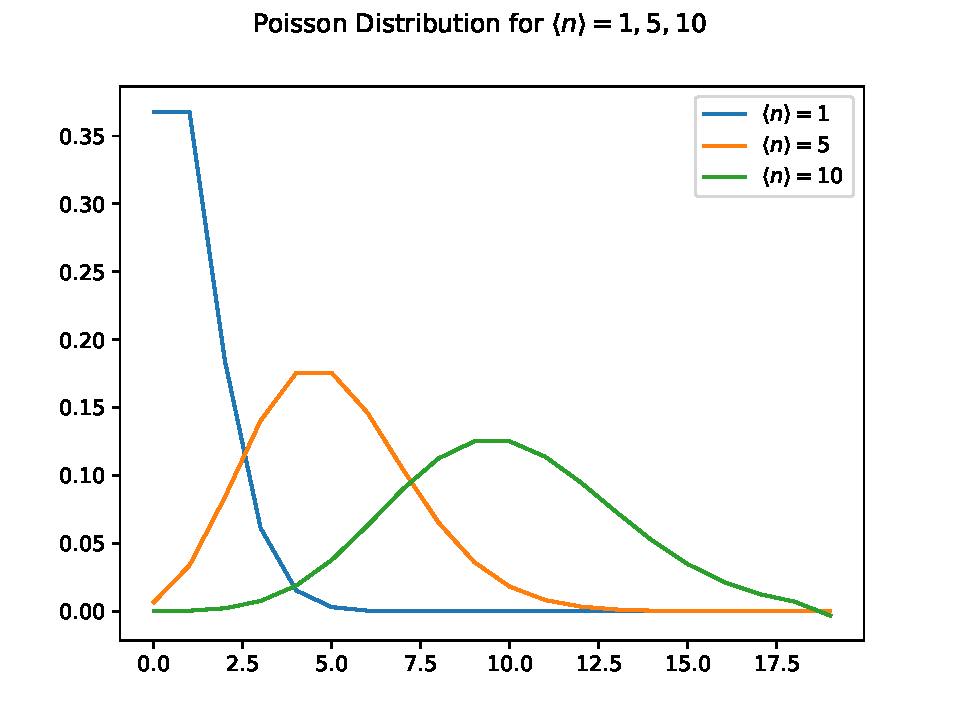
\includegraphics[width=0.7\textwidth]{/home/dj-lawton/Documents/Junior Sophister/Computer Simulation/Numerical Methods/Assignment 4/poisson.pdf}
    \caption{\label{fig: poisson} The Poisson distribution for $\braket{n}=1, 3, 5$. Note that the distribution peaks at or around the mean value, which is calculated in the code, and spreads out more for larger values of $\braket{n}$.}
\end{figure}
We can see that our first expression for the Poisson distribution, in Eq. \ref{fig: poisson} is the one that best fits the description of the dart throwing problem, as we have a fixed number of attempts, and a fixed probability of success per region.\\
\indent In this experiment, we run many simulations. After we sum together all our results, it is required to renormalise our distribution. This is required so that the sum of probabilities of hitting each region on each dart throw is 1. In each attempt we find a non-normalised distribution $h_1(n)$, $h_2(n)$, $h_3(n)$, etc. We then sum these distributions to get the total distribution $H(n)$, and then renormalise this distribution as described in Eq. \ref{eq: renormalisation}.
\begin{equation}
    \label{eq: renormalisation}
    P_{norm}(n) = \frac{H(n)}{\sum_{n=0}^{N}H(n)} = \frac{H(n)}{LT}, \quad \text{ where } H(n) = \sum_{i=1}^{N}h_i(n)
\end{equation}

\section{Method}
The random numbers were generated using the python library \texttt{random}, which uses the Mersenne Twister algorithm, whose name is derived from its use of Mersenne primes as its period lengths.\\
\indent The method for this experiment relies on the generation of pseudo-random numbers as described. We generate a random number between 1 and $L$, and increment the count of the element in the array that the dart `lands' in. This simulates one `dart-throw', so we repeat this process $N$ times. We then count the number of regions which have been hit $n$ times, for $n\leq N$. We can then evaluate the standard deviation and variance of this distribution. \\
\indent Instead of running the simulation once, we run it many times (10, 100, 1000, 10000) and sum the result. Since we require a probability distribution, we renormalise the result by dividing by the number of runs, times the number of regions on the board. This is then plotted and compared to to the shape of the previously described Poisson distribution. We then analyse the values over which our distribution probes the Poisson distribution, we say it probes the Poisson distribution for any $n$ values with non-zero probabilities (where the logarithm is not divergent). The experiment is repeated for varied $L$ values, and the results are observed.\\

\section{Results}

For this experiment, we fixed the total number of throws per experiment to 50.\\
The first result produced corresponds to our use of the Poisson distribution. For the distribution outlined in Eq. \ref{eq: poisson}, we measured the total probability to ensure normalisation, the mean of $n$, $\braket{n}$, then mean of $n^2$, $\braket{n^2}$, and the variance of $n$, $\sigma^2$, which we use to get the standard deviation $\sigma$. This is doen by summing over the following expressions,
\begin{align*}
    P_tot &= \sum_{n=0}^{N} P(n) (=1 \text{ if normalised.})\\
    \braket{n} &= \sum_{n=0}^{N} nP(n)\\
    \braket{n^2} &= \sum_{n=0}^{N} n^2P(n)\\
    \sigma^2 &= \braket{n^2} - \braket{n}^2\\
    \sigma &= \sqrt{\sigma^2}
\end{align*}
The results of this, for $\braket{n} = 1, 5, 10$ are shown in table \ref{tab: poisson values}.\\ 
\begin{table}[H]
    
    \centering
    \begin{tabular}{c|c|c|c|c|c}
        \hline
        ~ & $P_tot$ & $\braket{n}$ & $\braket{n^2}$ & $\sigma^2$ & $\sigma$\\
        \hline
        1 & 1.0 & 1.0 & 2.0 & 1.0 & 1.0\\
        5 & 1.0 & 4.999... & 29.999... & 5.0 & 2.236...\\
        10 & 0.999... & 9.999... & 110.0 & 10.0 & 3.162...\\
        \hline
    \end{tabular}
    \caption{\label{tab: poisson values} We can see that the values of $\braket{n}$ agree with the inputted values, and that the variation equals the mean. The standard deviation is also calculated, and we can see that it, as follows from the previous statement, is the square root of the mean.}
\end{table}

\indent Our second result is the distribution of the number of hits per region, for $L=100$, $N=50$. We ran the simulation 100, 1000, and 10000 times, and plotted the results.
\begin{figure}[H]
    \centering
    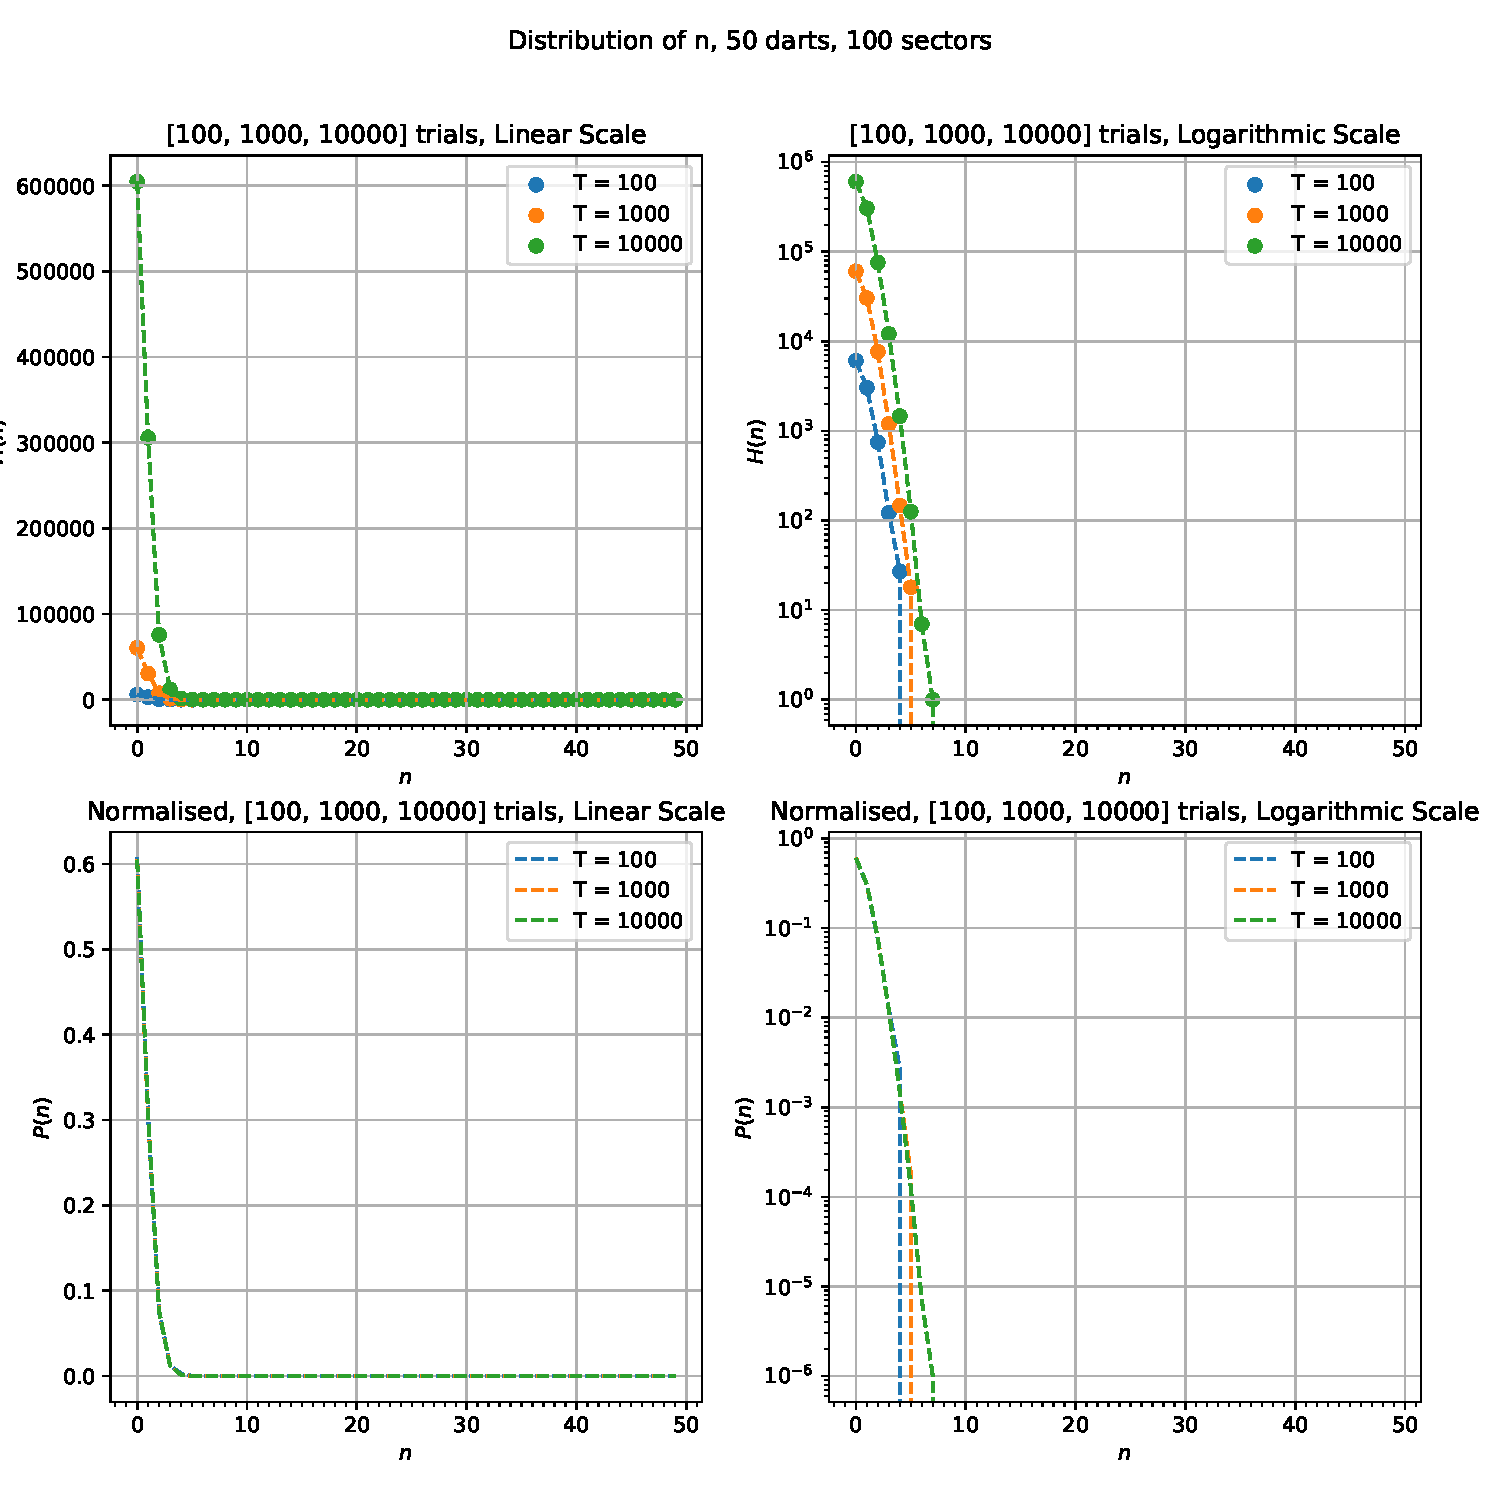
\includegraphics[width=0.9\textwidth]{/home/dj-lawton/Documents/Junior Sophister/Computer Simulation/Numerical Methods/Assignment 4/dart_throwingT[100, 1000, 10000]N50L100.pdf}
    \caption{\label{fig: 100_50_10} The distribution of the number of hits per region for $L=100$, $N=50$, 10 runs. Clearly, running a larger number of simulations probes the distribution to a higher degree. We can see that increasing the magnitude of the number of runs by about an order of magnitude allows the experiment to probe the Poisson distribution to approx. 1 higher $n$ value (The logarithmic plot diverges at higher $n$ values for larger $T$). It probes between $n=0$ and $n=7$ for $T=10000$.}
\end{figure}
The distribution in figure \ref{fig: 100_50_10} is clearly Poissonian, and shares a similar shape to a Poisson distribution with a mean less than 1. We can calculate the mean, and we see that it is exactly a half, or $\frac{N}{L}$. This is as expected, since the probability of hitting each region is $\frac{1}{L}$, and we have $N$ throws.\\
\indent As is produced by the code, one can see that the smallest probabilities for a given $n$ which are computed decrease massively with the magnitude of the number of runs. For example the smalles value on the $T = 10000$, $L = 100$ run, the smallest value was on the magnitude of $10^-6$, whereas for the $T = 100$ run, the smallest value was on the magnitude of $10^-4$.\\
\indent When the experiment was repeated for $L=5$, $N=50$, the results were as follows. The distribution was plotted as below,
\begin{figure}[H]
    \centering
    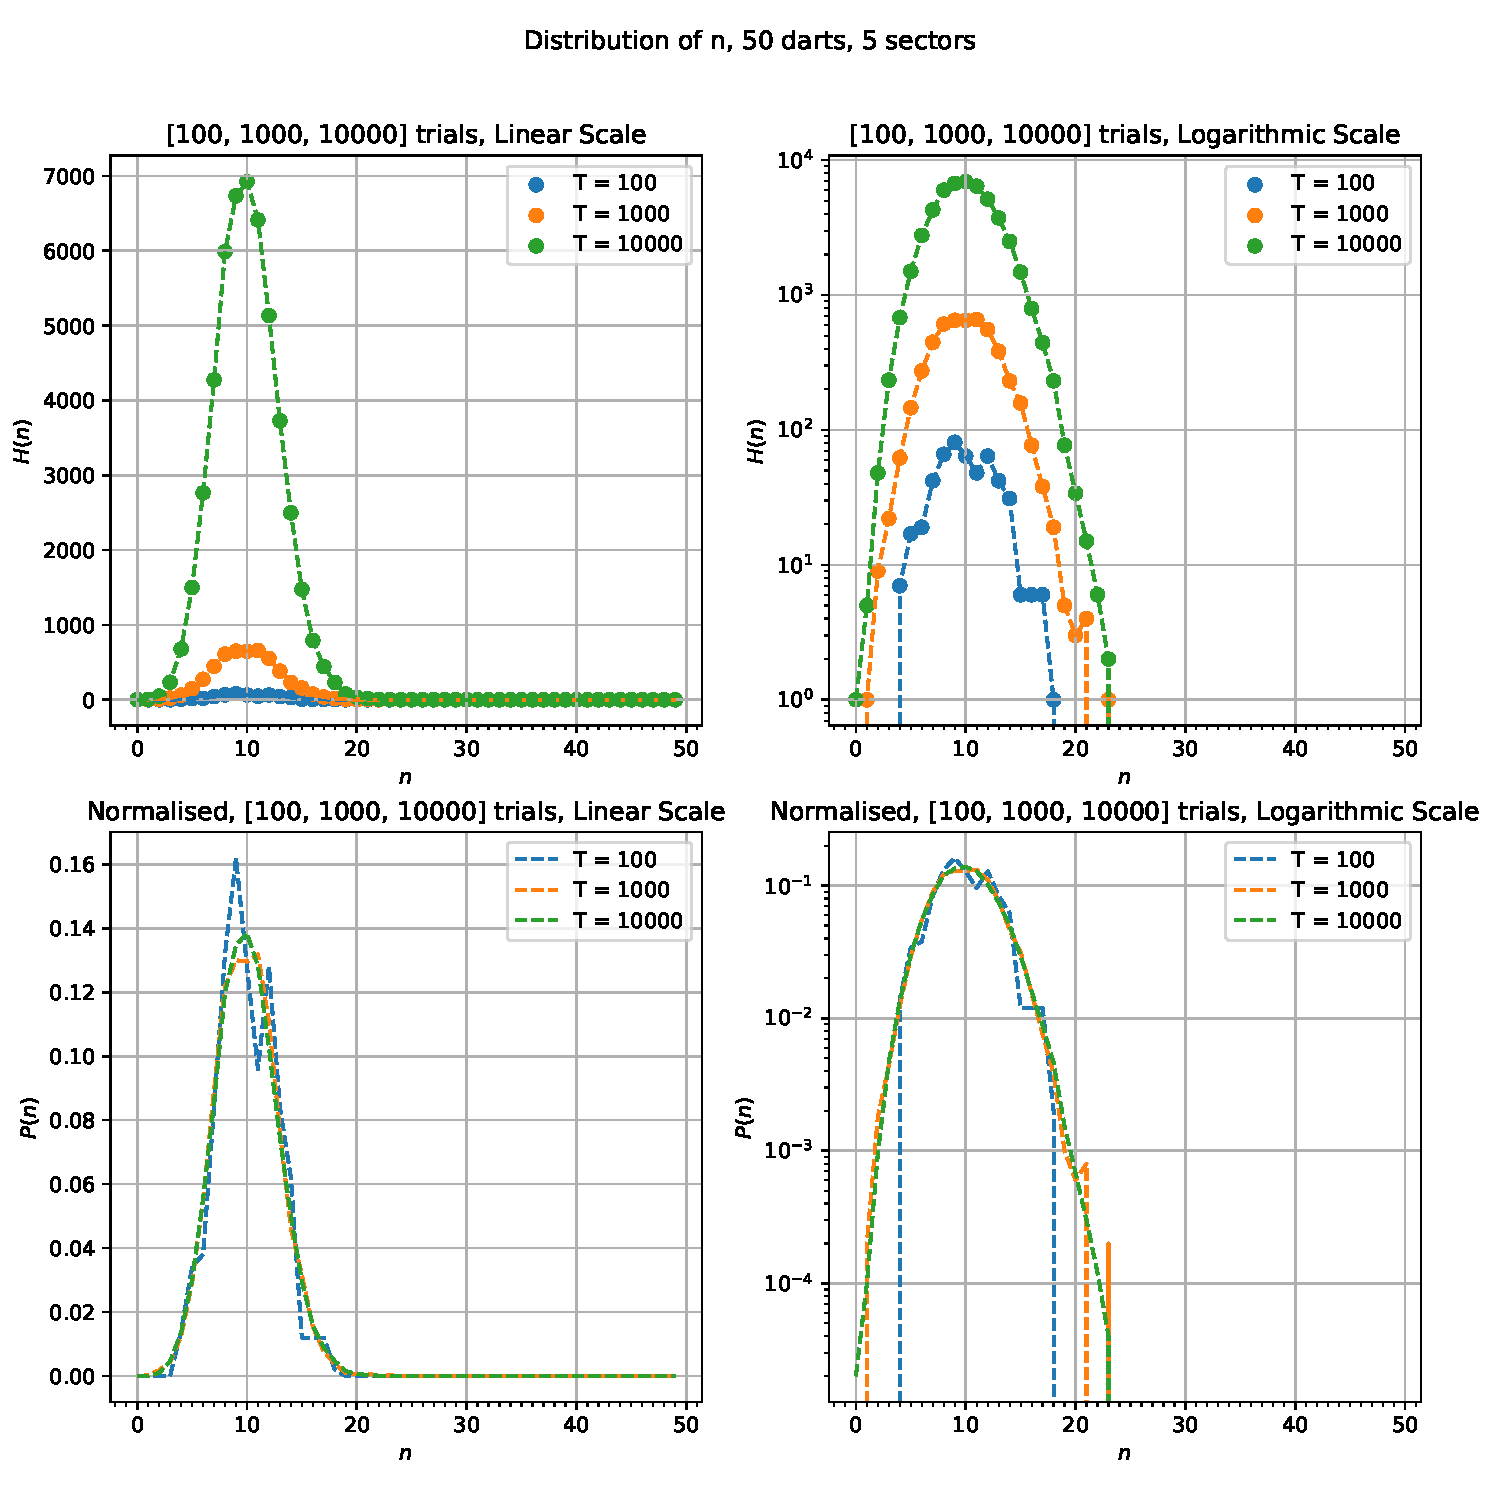
\includegraphics[width=0.9\textwidth]{/home/dj-lawton/Documents/Junior Sophister/Computer Simulation/Numerical Methods/Assignment 4/dart_throwingT[100, 1000, 10000]N50L5.pdf}
    \caption{\label{fig: 5_50_10} The distribution of the number of hits per region for $L=5$, $N=50$. We can see that the distribution is more spread out and the mean is larger than previously.}
\end{figure}
The mean of this distribution was calculated to be 10.0, which is as expected, since the mean is $\frac{N}{L}=10$. It is far more evident in the normalised plot here that the lower $T$ computations produce far less smooth distributions. It is also far easier to see the range over which the computation probes the Poisson distribution, which is much larger than the previous configuration, ranging from 0 to 23, for $T = 10000$. The smallest probabilities produced however are 0.002 for $T = 100$, 0.0001 for $T = 10000$, much larger than \\
\indent To conclude, the Poisson distribution is a good fit for the dart throwing problem, modelling especially well large $L$,$N$ values. It is also clear from the $L=5$ case, that for low $L$ values, the distribution converges less quickly (in $T$) to the smooth distribution. The change in the mean is due solely to the ratio of $N$ to $L$.\\
\end{document}